%! TEX program = xelatex
\documentclass[12pt]{octavo}
\usepackage[a4paper,margin=1in]{geometry}
\usepackage[localfonts=true]{tenth-sirawit}
\usepackage{tocloft}

\DeclareMathOperator*{\xor}{\texttt{XOR}}
\DeclareMathOperator{\spn}{span}

\setlength\cftparskip{-4pt}
\setlength\cftbeforesecskip{0pt}
\setlength\cftaftertoctitleskip{1pt}
\renewcommand{\contentsname}{\hfill\bfseries\huge\sffamily สารบัญ\hfill}
\renewcommand{\cftloftitlefont}{\sffamily}
\renewcommand{\cftlottitlefont}{\sffamily}
\renewcommand{\cftchapfont}{\sffamily}
\renewcommand{\cftsecfont}{\sffamily}
\renewcommand{\cftsubsecfont}{\sffamily}
\renewcommand{\cftchappagefont}{\sffamily}
\renewcommand{\cftsecpagefont}{\sffamily}
\renewcommand{\cftsubsecpagefont}{\sffamily}

\definecolor{gray75}{gray}{0.75}
\newcommand{\hsp}{\hspace{20pt}}
\titleformat{\chapter}[hang]{\Huge\bfseries\sffamily}{\thechapter\hsp\textcolor{gray75}{|}\hsp}{0pt}{\Huge\bfseries}
\titlespacing*{\chapter}{0pt}{-30pt}{20pt}

\title{101 for IOI}
\author{สิรวิชญ์ พงศ์นคินทร์}
\date{}

\begin{document}

\thispagestyle{titlepage}
\setstretch{1.3}

\vspace*{\fill}

\begin{center}
{
    \noindent\sffamily
    {\Huge\sbseries 101 for IOI}
    
    \medskip
    
    โจทย์ที่เลือกมาสำหรับการฝึกฝนในค่ายอบรมคัดเลือกวิชาคอมพิวเตอร์\\
    สำหรับโครงการจัดส่งผู้แทนประเทศไทยไปแข่งคอมพิวเตอร์โอลิมปิกระหว่างประเทศ
    
    \bigskip
    
    (เฉพาะส่วนที่ 1)
    
    \vspace{2cm}
    
    25 มกราคม 2565
    
    \vspace{3cm}
    
    \textbf{สิรวิชญ์ พงศ์นคินทร์}
    
    รวบรวมและเรียบเรียง
}
\end{center}

\vspace*{\fill}

\newpage

\chapter*{คำนำ}
\addcontentsline{toc}{chapter}{คำนำ}

หนังสือเล่มนี้ จัดทำขึ้นเพื่อเป็นส่วนเสริมสำหรับการเรียนการสอนในโครงการจัดส่งผู้แทนประเทศไทยไปแข่งขันโอลิมปิกระหว่างประเทศ วิชาคอมพิวเตอร์ ของ สถาบันส่งเสริมการสอนวิทยาศาสตร์และเทคโนโลยี (สสวท.)

เนื่องด้วยสถานการณ์ที่ไม่เป็นระเบียบเรียบร้อยของไม่กี่ปีที่ผ่านมา ซึ่งเป็นผลกระทบจากเหตุการณ์การระบาดของโรคติดเชื้อไวรัสโคโรนา 2019 (COVID-19) ทำให้การจัดการเรียนการสอนภายในค่ายเตรียมความพร้อมหลายครั้งเสียประสิทธิภาพ ผู้เขียนได้เขียนหนังสือเล่มนี้โดยมีวัตถุประสงค์ที่จะมาทดแทน หรือเสริมสร้าง ทักษะทางวิชาการ ซึ่งผู้เขียนมองว่าเป็นองค์ประกอบสำคัญสำหรับการเตรียมความพร้อมผู้เรียนไปแข่งขันคอมพิวเตอร์โอลิมปิกระหว่างประเทศ

เนื่องจากผู้เรียนบางคนประสบปัญหาทางภาษา ผู้เขียนจึงพยายามเขียนหนังสือเล่มนี้ให้อยู่บนพื้นฐานของภาษาไทยมากที่สุดเท่าที่จะทำได้ หนังสือเล่มนี้เหมาะสำหรับผู้อ่านที่เป็นนักเรียน (โดยเฉพาะนักเรียนค่ายคอมพิวเตอร์โอลิมปิกทุกระดับ) และผู้สนใจศึกษาทั่วไป ผู้เขียนหวังว่าผู้อ่านจะได้รับประโยชน์จากการอ่าน (และที่สำคัญคือการทำโจทย์) จากหนังสือเล่มนี้กลับไปไม่มากก็น้อย

ในขณะที่ผู้เขียนได้ทำการรวบรวมหนังสือเล่มนี้ ผู้เขียนขอยืนยันว่าไม่มั่นใจในความสามารถตนเอง กล่าวคือ หนังสือเล่มนี้อาจมีข้อผิดพลาดประการใดก็เป็นได้ ผู้เขียนขอขอบคุณล่วงหน้าสำหรับทุกคำติชม หากผู้อ่านพบข้อผิดพลาดประการใด สามารถติดต่อผู้เขียนกลับมาได้ที่อีเมล sirawit@pongnakin.com

ผู้เขียนขอแสดงความขอบคุณต่อ คุณอาภาพงศ์ จันทร์ทอง และคุณพงศพล พงศาวกุล สำหรับแม่แบบ (template) สำหรับการพิมพ์หนังสือเล่มนี้ นอกจากนี้ขอแสดงความขอบคุณต่อ อาจารย์ ผศ.ดร.จิตร์ทัศน์ ฝักเจริญผล และ อาจารย์ ผศ.ดร.นัทที นิภานันท์ สำหรับการช่วยเหลือดูแลนักเรียนในค่ายเตรียมความพร้อม

\chapter*{LICENSE}
\addcontentsline{toc}{chapter}{LICENSE}

For the section \ref{codeforces:786B} the following license is applied:
\begin{center}
\textbf{Codeforces materials usage license (v. 0.1)}    
\end{center}
\begin{enumerate}
    \item You may publish the texts of Codeforces problems in any open sources, but you must preserve a direct link to the site http://codeforces.ru (http://codeforces.com for English statements) and indicate Codeforces as the problem source. These data should be located in the close proximity to the statement, be easily noticeable and readable. It is forbidden to publish Codeforces problems in open sources supporting automatic testing (such as online judges or similar resources).
    \item You must not use tests and other materials of the problems (generators, checkers, validators) to publish tasks in open sources supporting automatic testing (such as online judges or similar resources) even provided the original problem conditions has been changed.
    \item You may use the provided material: tests, generators, checkers, validators and others for individual training or to organize short-term teaching and training activities with the participants present on-site. Task conditions should contain the data from paragraph 1 of this license. The secondary (subsequent) distribution of the tasks should contain this license and comply fully with the license’s rules.
\end{enumerate}

For the sections denoted with a direct reference to the author, refer to the author for direct license.

For all other sections (with no direct reference), the following license is applied:

This work is licensed under the Creative Commons Attribution-NonCommercial 4.0 International License. To view a copy of this license, visit
http://creativecommons.org/licenses/by-nc/4.0/.

\begin{center}

\includegraphics[width=4cm]{by-nc}
\end{center}

\newpage

{
\sffamily
\tableofcontents
}

\part{\sffamily แบบฝึกหัดส่วนที่ 1}
\pagestyle{plain}
\fancyhead[R]{\sffamily {\leftmark}}
\chapter{Complexity Analysis, Sorting \& Searching}

\section{A Big Factorial}

\begin{exercise}
ให้ $g \colon \N \to \R$ นิยามโดย $g(n) = \log(n!)$ สำหรับ $n \in \N$ ใด ๆ จงแสดงว่า $g(n) \in \Theta(n \log n)$
\end{exercise}

\section{An Impossible Problem}
\label{twitter:willmcgugan1}
กำหนดให้มีอาเรย์ของจำนวนเต็มที่อาจเป็น 0, 1 หรือ 2 ก็ได้ ขนาด $n$ เช่น $[0, 1, 2, 0, 1]$

จงออกแบบอัลกอริทึมที่จะแบ่งอาเรย์นี้เป็นสองส่วนโดยการตัดออกเป็นส่วนที่ติดกันทางซ้าย เรียกว่า $A$ และส่วนที่ติดกันทางขวา เรียกว่า $B$ โดยมีเงื่อนไขว่า ผลรวมของจำนวนใน $A$ จะต้องมีค่าเท่ากับ $X$ และ $B$ จะต้องไม่เริ่มต้นด้วย $0$ (เพื่อความง่ายขอรับประกันว่ามีคำตอบแน่นอน)

โดยอัลกอริทึมจะต้องมีประสิทธิภาพ กล่าวคือ ทำงานได้เร็วกว่า $O(n)$

\begin{exercise}
จงพิสูจน์ว่ามันทำไม่ได้ กล่าวคือ สำหรับอัลกอริทึมใด ๆ ก็ตามที่สามารถแก้ปัญหาข้างต้นได้ อัลกอริทึมนั้นจะต้องใช้เวลา $\Omega(n)$ (Hint: พิจารณาเฉพาะเงื่อนไขของ $B$)
\end{exercise}

\begin{exercise}
สมมติว่าตัดเงื่อนไขของ $B$ ออก เหลือเพียงเงื่อนไขว่าผลรวมของจำนวนใน $A$ จะต้องมีค่าเท่ากับ $X$ จงแสดงว่าอัลกอริทึมที่แก้ปัญหานี้ได้จะต้องใช้เวลา $\Omega(n)$
\end{exercise}

\noindent \textbf{หมายเหตุ.} โจทย์ดัดแปลงมาจาก \\ \url{https://twitter.com/willmcgugan/status/1459233690052141063?s=20}

\section{Sieve of Eratosthenes}

สำหรับจำนวนเต็มบวก $N$ พิจารณาอัลกอริทึมที่ตรวจสอบว่าจำนวนใดบ้างเป็นจำนวนเฉพาะตั้งแต่ $1$ ถึง $N$ ดังนี้

\begin{lstlisting}
bool is_prime[N+1];
is_prime[1] = false;
for(int i = 2; i <= N; i++){
    is_prime[i] = true;
}
for(int gap = 2; gap <= N; gap++){
    for(int i = 2*gap; i <= N; i += gap){
        is_prime[i] = false;
    }
}
\end{lstlisting}

\begin{exercise}
สังเกตว่า การวนซำ้ชั้นในจะทำเพียง $O\left(\frac{N}{\texttt{gap}}\right)$ รอบ ดังนั้นเวลารวมของอัลกอริทึมนี้จึงเป็น
\[
O\left(\sum_{\texttt{gap}=2}^N \frac{N}{\texttt{gap}}\right)
\]
จงพิสูจน์ว่า เวลารวมของอัลกอริทึมนี้ อยู่ใน $O(N \log N)$
\end{exercise}

\begin{bonus}
การดัดแปลงอัลกอริทึมข้างต้น ให้สนใจเฉพาะกรณีที่ \texttt{gap} เป็นจำนวนเฉพาะ สามารถทำให้เวลาที่อัลกอริทึมนี้ใช้ดีขึ้นไปอีก จงหาเวลาที่ใช้และพิสูจน์
\end{bonus}
\chapter{Mathematical Proof and Induction}

\section{Infinite Number of Primes in an Arithmetic Progression}

\begin{exercise}
จงพิสูจน์ว่ามีจำนวนเฉพาะอยู่เป็นอนันต์ตัว
\end{exercise}

\begin{exercise}
จงพิสูจน์ว่ามีจำนวนเฉพาะอยู่เป็นอนันต์ตัวที่อยู่ในรูป $4k+3$ เมื่อ $k$ เป็นจำนวนเต็ม
\end{exercise}

\section{Well-Ordering Principle and Principle of Mathematical Induction}

สำหรับส่วนนี้ ให้ $\N$ แทนเซตของจำนวนเต็มไม่ลบ คือ $\{0, 1, 2, \dots\}$

\begin{exercise}
ตามสัจพจน์พื้นฐานของจำนวนนับ เราสามารถใช้การอุปนัยเชิงคณิตศาสตร์ได้ จงพิสูจน์หลักการจัดอันดับดีแล้ว ซึ่งกล่าวไว้ว่า สำหรับเซต $S \subseteq \N$ ใด ๆ ที่ $S \ne \emptyset$ จะได้ว่า $S$ มีสมาชิกน้อยสุด
\end{exercise}

\begin{exercise}
สมมติว่าเราไม่เชื่อหลักการอุปนัยเชิงคณิตศาสตร์ แต่มั่นใจว่าหลักการจัดอันดับดีเป็นจริง จงพิสูจน์หลักการอุปนัยเชิงคณิตศาสตร์ กล่าวคือ จงพิสูจน์ว่าสำหรับเซต $K \subseteq \N$ ใด ๆ หาก $0 \in K$ และสำหรับทุกจำนวนเต็มไม่ลบ ถ้า $n \in K$ แล้ว $n+1 \in K$ เราจะสามารถสรุปได้ว่า $\N = K$
\end{exercise}

\section{Sheep Paradox}

\begin{exercise}
สมมติว่าแกะทุกตัวมีสีอยู่ประจำตัวสีเดียว กล่าวคือไม่มีแกะตัวใดที่มีสีสองสีในตัวเดียวกัน พิจารณาการให้เหตุผลดังต่อไปนี้ เพื่อพิสูจน์ว่า "แกะทุกตัวบนโลกมีสีเดียวกัน" ด้วยการอุปนัยเชิงคณิตศาสตร์

\begin{proof}
ขั้นฐาน สมมติว่ามีแกะอยู่ตัวเดียว แกะตัวนั้นย่อมมีสีเดียว ทำให้เซตของแกะทุกเซตขนาด $1$ ประกอบด้วยแกะสีเดียวกัน

ขั้นอุปนัย สมมติให้ $n$ เป็นจำนวนเต็มบวก และสมมติว่าเซตของแกะทุกเซตขนาด $n$ ประกอบด้วยแกะสีเดียวกันทั้งนั้น เราจะแสดงว่าเซตของแกะทุกเซตขนาด $n+1$ ก็ประกอบด้วยแกะสีเดียวกันทั้งนั้น โดยอาศัยว่าพิจารณาเซตของแกะ $n+1$ ตัว เราสามารถหยิบแกะออกไปตัวหนึ่ง จะได้ว่าแกะที่เหลือมีสีเดียวกันเพราะเป็นเซตขนาด $n$ เมื่อใส่แกะตัวเดิมกลับเข้าไปแล้วเอาแกะตัวอื่นออก ก็จะได้ว่าแกะที่เหลือมีสีเดียวกันเพราะเป็นเซตขนาด $n$ จึงสรุปได้ว่าแกะทั้ง $n+1$ ตัวมีสีเดียวกัน

จากหลักการอุปนัยเชิงคณิตศาสตร์ จึงสรุปได้ว่าสำหรับจำนวนเต็มบวก $n$ ใด ๆ แกะทั้ง $n$ ตัวมีสีเดียวกันเสมอ ให้ $N$ เป็นจำนวนแกะบนโลกใบนี้ เนื่องจาก $N$ เป็นจำนวนเต็มบวก จึงได้ว่าแกะทุกตัวบนโลกนี้มีสีเดียวกัน
\end{proof}

เกิดอะไรขึ้นกับบทพิสูจน์ข้างต้น บทพิสูจน์ข้างต้นถูกแล้วหรือ? หากผิด ผิดอย่างไร?
\end{exercise}

\section{A Fixed Point}

กำหนดให้ $f \colon [0, 1] \to [0, 1]$ เป็นฟังก์ชันซึ่ง สำหรับทุก $x, y \in [0, 1]$ หาก $x \leq y$ แล้ว $f(x) \leq f(y)$

นิยาม
\[
A := \{ x \in [0, 1] \colon x \leq f(x) \}
\]

เราจะกล่าวว่า สำหรับเซต $S \subseteq \R$ ใด ๆ $M$ จะเป็นขอบเขตบนของ $S$ ก็ต่อเมื่อสำหรับทุก $x \in S$, $x \leq M$

และเราจะกล่าวว่า สำหรับเซต $S \subseteq \R$ ใด ๆ $m$ จะเป็นขอบเขตบนน้อยสุดของ $S$ ก็ต่อเมื่อ $m$ เป็นขอบเขตบนของ $S$ และไม่มีขอบเขตบนอื่นใดของ $S$ ที่มีค่าน้อยกว่า $m$

\begin{exercise}
จงแสดงว่า $A$ มีขอบเขตบนน้อยสุดใน $[0, 1]$ (ซึ่งจะเขียนแทนด้วยสัญลักษณ์ $a$)
\end{exercise}

\begin{exercise}
จงแสดงว่า $f(a) \leq a$
\end{exercise}

\begin{exercise}
สำหรับ $\varepsilon > 0$ ใด ๆ จงพิสูจน์ว่า $a \leq f(a) + \varepsilon$
\end{exercise}

\begin{exercise}
จงพิสูจน์ว่ามีจำนวนจริง $z \in [0, 1]$ ที่ $f(z) = z$
\end{exercise}

\section{One-to-one Correspondence}

สำหรับส่วนนี้ ให้ $\N$ แทนเซตของจำนวนเต็มไม่ลบ คือ $\{0, 1, 2, \dots\}$

\begin{exercise}
จงหาฟังก์ชันหนึ่งต่อหนึ่งทั่วถึงจาก $\N$ ไปสู่ $\Z$ และพิสูจน์ความเป็นหนึ่งต่อหนึ่งและทั่วถึงของฟังก์ชันนั้น
\end{exercise}

\begin{exercise}
จงหาฟังก์ชันหนึ่งต่อหนึ่งทั่วถึงจาก $\Z$ ไปสู่ $\Q$ และพิสูจน์ความเป็นหนึ่งต่อหนึ่งและทั่วถึงของฟังก์ชันนั้น
\end{exercise}

\begin{exercise}
จงหาฟังก์ชันหนึ่งต่อหนึ่งทั่วถึงจาก $\N$ ไปสู่ $\N \times \N$ และพิสูจน์ความเป็นหนึ่งต่อหนึ่งและทั่วถึงของฟังก์ชันนั้น
\end{exercise}

\begin{bonus}
จงพิสูจน์ว่าไม่สามารถหาฟังก์ชันหนึ่งต่อหนึ่งจาก $\N$ ไปสู่ $\R$ ได้
\end{bonus}
\chapter{Tree \& Hash}

\section{Fenwick Tree}

ในปี 1994 นั้น Peter M. Fenwick ได้ออกแบบโครงสร้างข้อมูลที่มีชื่อว่า Binary Indexed Tree หรือที่เราเรียกกันว่า Fenwick Tree ในงานเขียนชื่อว่า ``A new data structure for cumulative frequency tables''

สำหรับการ implement โครงสร้างนี้ระหว่างเขียนโปรแกรมเชิงการแข่งขันในภาษา C++ หลายคนนิยมใช้วิธีดังต่อไปนี้

\begin{lstlisting}
int FT[M];
int lsb(int n){
    return n & -n;
}
void add(int idx, int amt){
    while(idx < M){
        FT[idx] += amt;
        idx += lsb(idx);
    }
}
int sum(int idx){
    int ret = 0;
    while(idx > 0){
        ret += FT[idx];
        idx -= lsb(idx);
    }
    return ret;
}
\end{lstlisting}

\begin{exercise}
สำหรับจำนวนเต็มบวก $n \in \N_{\texttt{int}}$ ใด ๆ เมื่อ $\N_{\texttt{int}}$ แทนเซตของจำนวนเต็มระหว่าง $0$ ถึง $2^{32}-1$ จงแสดงว่าหากเขียน $n$ ในรูป
\[
n = \sum_{n=0}^{31} b_i 2^i
\]
เมื่อ $b_i \in \{0, 1\}$ สำหรับ $i \in \{0, \dots, 31\}$ แล้ว \texttt{lsb(n)} จะมีค่าเท่ากับ $2^{\min\{i \in \{0, \dots, 31\} \colon b_i = 1\}}$
\end{exercise}

ให้ $M$ เป็นจำนวนเต็มที่ $10 \leq M \leq 2\,000\,000$

\begin{exercise}
จงพิสูจน์ว่า สำหรับ $n \in \N$ ใด ๆ ที่ $0 \leq n < M$ การเรียกใช้ฟังก์ชัน \texttt{sum(n)} จะไปพิจารณาค่าใน \texttt{FT} เพียง $O(\log M)$ ค่าเท่านั้น (คำใบ้: พิจารณาฟังก์ชัน $\phi \colon \N_{\texttt{int}} \to \N$ นิยามโดย สำหรับจำนวนเต็มบวก $n \in \N_{\texttt{int}}$ ใด ๆ หากเขียน $n$ ในรูป
\[
n = \sum_{n=0}^{31} b_i 2^i
\]
เมื่อ $b_i \in \{0, 1\}$ สำหรับ $i \in \{0, \dots, 31\}$ แล้ว นิยามให้ $\phi(n) = |\{i \in \{0, \dots, 31\} \colon b_i = 1\}|$ แล้วสังเกตค่าของ $\phi(n)$)
\end{exercise}

หากรับประกันว่าค่าที่ใส่ลงไปในฟังก์ชัน \texttt{add} แต่ละครั้งไม่มีครั้งใดติดลบ เราจะได้เงื่อนไขพิเศษว่า \texttt{sum(n)} มีค่ามากกว่าหรือเท่ากับศูนย์เสมอ สำหรับทุก $0 \leq n < M$

\begin{exercise}
จงพิสูจน์ข้อความข้างต้น
\end{exercise}

\begin{exercise}
กำหนดค่า $k$ ให้มา หากต้องการหาค่าของจำนวนเต็ม $n$ ที่น้อยที่สุดที่ \texttt{sum(n)} มีค่ามากกว่าหรือเท่ากับ $k$ จงออกแบบอัลกอริทึมที่ทำงานดังกล่าวได้อย่างมีประสิทธิภาพ (เป้าหมายคือ $O(\log M)$)
\end{exercise}

\section{Hashed Set}

โดยทั่วไป เราไม่สามารถประกาศใช้ \texttt{std::unordered\_set<std::set<int>>} ได้ เพราะโครงสร้างข้อมูล \texttt{std::set<int>} นั้นไม่นิยามแฮชฟังก์ชัน อย่างไรก็ตามหากเซตของเรานั้นเป็นเซตทางคณิตศาสตร์ที่มีสมาชิกคงที่ ไม่มีการใส่เข้าหรือลบออก มันก็ยังเป็นไปได้ที่จะออกแบบตารางแฮชสำหรับเซตเหล่านี้

\begin{exercise}
จงออกแบบแฮชฟังก์ชัน $h \colon \mathcal{P}(\N_{\texttt{int}}) \to \N$ เมื่อ $\N_{\texttt{int}}$ แทนเซตของจำนวนเต็มระหว่าง $0$ ถึง $2^{32}-1$ ที่มีประสิทธิภาพ และอธิบายว่าฟังก์ชันที่ออกแบบนี้ดีอย่างไร
\end{exercise}

\section{Merge Sort tree}

ปกติแล้ว เราสามารถใช้ Segment tree หรือ Interval tree ในการตอบคำถามประเภท Range Minimum Query (RMQ) คือ มีอาเรย์ของจำนวนเต็มใน $\N_{\texttt{int}}$ ประกอบด้วยจำนวนเต็ม $N$ ตัว เรียกว่า $A$ และจะเขียน $A_i$ แทนจำนวนเต็มในช่องที่ $i$ ของอาเรย์ สำหรับ $i \in \{0, \dots, N-1\}$ แล้วมีคำถามต่อมาอีก $Q$ คำถาม แต่ละคำถามจะให้ค่า $(l, r) \in \{0, \dots, N-1\}^2$ มา จงหาว่าค่าต่ำสุดในช่วงจากช่องที่ $l$ ถึงช่องที่ $r$ เป็นเท่าใด กล่าวคือ ให้หาค่าของ $\min\{A_i \colon i \in [l, r] \cap \N\}$

เรารู้ว่าโครงสร้างอย่าง Segment tree หรือ Interval tree สามารถตอบคำถามดังกล่าวได้ในเวลา $O(\log N)$ อย่างไรก็ตาม ในข้อนี้เราจะพูดถึงคำถามอีกประเภทที่จะต้องใช้โครงสร้างข้อมูลที่ดัดแปลงมากจากต้นไม้เหล่านั้น

\textbf{โจทย์} มีอาเรย์ของจำนวนเต็มใน $\N_{\texttt{int}}$ ประกอบด้วยจำนวนเต็ม $N$ ตัว เรียกว่า $A$ และจะเขียน $A_i$ แทนจำนวนเต็มในช่องที่ $i$ ของอาเรย์ สำหรับ $i \in \{0, \dots, N-1\}$ แล้วมีคำถามต่อมาอีก $Q$ คำถาม แต่ละคำถามจะให้ค่า $(l, r, x) \in \{0, \dots, N-1\}^2 \times \N_{\texttt{int}}$ มา ให้หาว่าในช่วงระหว่างช่องที่ $l$ ถึงช่องที่ $r$ นั้นมีค่าอยู่กี่ตัวที่ไม่เกิน $x$ กล่าวคือ ให้หาค่าของ $|\{A_i \colon i \in [l, r] \cap \N \text{ และ } A_i \leq x\}|$

\begin{exercise}
มีวิธีการในตอบคำถามในโจทย์ข้างต้นโดยทำการเตรียมการ (preprocess) ใน $O(N \log N)$ ใช้หน่วยความจำใน $O(N \log N)$ และตอบคำถามใน $O(\log^2 N)$ หรือไม่ หากมี จงอธิบายและพิสูจน์ว่าทำได้ตามเป้าหมายทุกอย่าง
\end{exercise}

พิจารณาปัญหาต่อมา โดยโจทย์มีดังนี้

\textbf{โจทย์} มีอาเรย์ของจำนวนเต็มใน $\N_{\texttt{int}}$ ประกอบด้วยจำนวนเต็ม $N$ ตัว เรียกว่า $A$ และจะเขียน $A_i$ แทนจำนวนเต็มในช่องที่ $i$ ของอาเรย์ สำหรับ $i \in \{0, \dots, N-1\}$ แล้วมีคำถามต่อมาอีก $Q$ คำถาม แต่ละคำถามจะให้ค่า $(l, r, c) \in \{0, \dots, N-1\}^3$ มา และรับประกันว่า $c$ มีค่าไม่เกิน $|r-l|$ ให้หาว่าในช่วงระหว่างช่องที่ $l$ ถึงช่องที่ $r$ หากนำมาเรียงจากน้อยไปมากแล้ว ตัวที่ $c$ จากน้อยไปมาก (เริ่มนับจาก $0$ ถึง $r-l$) จะมีค่าเท่ากับเท่าไร

\begin{exercise}
จงออกแบบอัลกอริทึม/โครงสร้างข้อมูลที่ทำตามโจทย์ข้างต้นโดยทำการเตรียมการใน $O(N \log N)$ ใช้หน่วยความจำใน $O(N \log N)$ และตอบคำถามข้างต้นได้ใน $O(\log^3 N)$
\end{exercise}

\begin{bonus}
มีวิธีที่ตอบคำถามได้เร็วกว่า $O(\log^3 N)$ หรือไม่?
\end{bonus}

\section{Prime Probing}

\begin{exercise}
สำหรับตารางแฮชบรรจุจำนวนเต็มไม่ลบขนาด $10$ ซึ่งนับเป็นช่องตั้งแต่ช่องที่ $0$ ถึงช่องที่ $9$ เราจะมีอัลกอริทึมการใส่ของในตารางแฮชแบบ Prime Probing ดังนี้

สำหรับการใส่จำนวนเต็มไม่ลบ $n$ ลงไปในตารางแฮช ให้ $r$ เป็นเลขหลักหน่วยของ $n$ หลังจากนั้นพิจารณาช่อง $r$ ของตาราง สำหรับ $i = 1, 2, 3, \dots$ หากในช่องที่ $r$ นั้นมีของอยู่ ให้ปรับ $r$ กลายเป็นเลขหลักหน่วยของ $(r+p_i)$ แล้วทำไปเรื่อย ๆ จนกว่าช่อง $r$ จะว่าง แล้วจึงนำ $n$ ใส่ลงในช่อง $r$ เมื่อ $p_i$ แทนจำนวนเฉพาะตัวที่ $i$ ($p_1 = 2; p_2 = 3; \dots$)

จงเขียนผลลัพธ์ของตารางแฮชหลังดำเนินการแต่ละอย่างต่อไปนี้ (ทีละอย่าง)

\begin{enumerate}[nosep,label={\bfseries (\roman*)}]
    \item ใส่ $42$
    \item ใส่ $69$
    \item ใส่ $112$
    \item ใส่ $116$
    \item ใส่ $44$
    \item ใส่ $2022$
\end{enumerate}
\end{exercise}

\begin{exercise}
ระหว่างวิธีการจัดการ Hash collision แบบ Probing กับแบบใช้โครงสร้างข้อมูลภายในซ้อนลงไป สอบแบบนี้ต่างกันอย่างไร และมีข้อดีข้อเสียอย่างไร?
\end{exercise}
\chapter{Divide and Conquer}

\section{Van Emde Boas Tree Analysis}

ในปี 1975 ทีมของนักวิทยาศาสตร์คอมพิวเตอร์ นำโดยชาวดัตช์คนหนึ่ง ชื่อของเขาคือ Peter van Emde Boas เขาได้ทำการออกแบบโครงสร้างข้อมูลชนิดหนึ่งขึ้นมา ปัจจุบันนี้มีชื่อเรียกว่า van Emde Boas tree

โดยต้นไม้ชนิดนี้ สามารถทำหน้าที่ได้เทียบเท่าโครงสร้างข้อมูลประเภทตารางค้นหา (lookup table) แต่ในที่นี้เราจะพูดถึงรูปแบบที่ใช้ทำหน้าที่เก็บข้อมูลประเภทเซตของจำนวนเต็มไม่ลบขนาด $m$ บิต (ข้อมูลมีค่าระหว่าง $0$ ถึง $2^m-1$)

สำหรับในข้อนี้ เราจะไม่อธิบายขั้นตอนวิธีการทำงานของโครงสร้างข้อมูล van Emde Boas tree เนื่องจากเป็นเนื้อหานอกขอบเขต (จะอยู่ในขอบเขตค่ายถัดไป) อย่างไรก็ตาม เป้าหมายของข้อนี้คือการพิสูจน์ Time Complexity ของการทำงานบน van Emde Boas tree ในแต่ละครั้ง

\begin{exercise}
กำหนดให้ $R \colon \N \to \R$ นิยามโดย $R(1) = R(0) = 1$ และ 
\[
R(n) = R\left(\left\lfloor\frac{n}{2}\right\rfloor\right) + O(1)
\]
สำหรับ $n \in \N - \{0, 1\}$ ใด จงแสดงว่า $R(n) \in O(\log n)$
\end{exercise}

กำหนดให้ $T \colon \R \to \R$ โดย $T(x) = 0$ สำหรับทุกจำนวนจริง $x < 1$ และ $T(1) = 1$

ต้นไม้ van Emde Boas ที่สามารถเก็บจำนวนเต็มได้ตั้งแต่ $0$ ถึง $M-1$ เมื่อ $M$ เป็นผลยกกำลังของสอง (กล่าวคือ $M = 2^m$ สำหรับบาง $m \in \N$) จะใช้ระยะเวลาในการดำเนินการหนึ่งครั้งในเวลา $T(M)$ เมื่อ
\[
T(x) = T(\sqrt{x}) + O(1)
\]
สำหรับจำนวนจริง $x > 1$ ใด ๆ

\begin{exercise}
จงพิสูจน์ว่า $S(m) \in O(\log m)$ เมื่อ $S \colon \R \to \R$ เป็นฟังก์ชันนิยามโดย $S(x) := T(2^x)$
\end{exercise}

\begin{exercise}
จงพิสูจน์ว่า $T(M) \in O(\log \log M)$
\end{exercise}

\section{Centroid Decomposition of a Tree}

พิจารณาต้นไม้ที่ประกอบด้วยจุดยอด $N$ จุดยอด (มีเส้นเชื่อม $N-1$ เส้นเชื่อมตามนิยามของต้นไม้)

\begin{exercise}
จงพิสูจน์ว่ามีจุดยอดอย่างน้อยหนึ่งจุด ที่เมื่อตัดจุดยอดนี้ออกไปแล้วจะแบ่งต้นไม้ออกเป็น $k$ ส่วน โดยที่ต้นไม้ย่อยแต่ละส่วนจากทั้ง $k$ ส่วน จะมีจำนวนจุดยอดในต้นไม่้ย่อยนั้นไม่เกิน $\frac{N}{2}$
\end{exercise}

เราทำการสร้างต้นไม้ใหม่อีกต้น เรียกว่า Centroid Tree โดยมีวิธีการสร้างดังนี้:

\begin{enumerate}[nosep]
    \item จากต้นไม้ต้นปัจจุบัน ให้ $c$ เป็น centroid ของต้นไม้นี้
    \item ตัด $c$ ออกจากต้นไม้ปัจจุบัน ทำให้ต้นไม้หลักแบ่งออกเป็น $k$ ต้นไม้ย่อย หลังจากนั้นทำการหา centroid ของต้นไม้ย่อยแต่ละต้น เรียกเป็น $c_1, c_2, \dots, c_k$
    \item ทำการเชื่อมเส้นเชื่อมบน Centroid Tree โดยสร้างเส้นเชื่อม $(c, c_1), (c, c_2), \dots, (c, c_k)$ และกำหนดให้ $c$ เป็น parent ของ $c_1, c_2, \dots, c_k$ ใน Centroid Tree
    \item ย้อนกลับไปทำข้อ 1. โดยเปลี่ยนต้นไม้ปัจจุบันเป็นต้นไม้ย่อยแต่ละต้นที่ถูกตัดออกจาก $c$
\end{enumerate}

โดยให้ centroid เริ่มแรกเป็นรากของ Centroid Tree

\begin{exercise}
จงพิสูจน์ว่าความสูงของ Centroid Tree อยู่ใน $O(\log N)$
\end{exercise}

นอกจากนี้ โดยปกติการทำการค้นหาแนวลึก (Depth-first search) บนต้นไม้ จะใช้เวลา $O(N)$ โดยคิดเวลาดังนี้
\[
T(t_i) = \sum_{u \in C(t_i)} T(t_u) + O(1)
\]
เมื่อ $t_i$ แทนต้นไม้ย่อยที่มีรากอยู่ที่ $i$ และ $C(x)$ แทนเซตของลูก (children) ของจุดยอด $x$

การทำงานของการค้นหาแนวลึกข้างต้นใช้เวลา $O(N)$ อย่างไรก็ตาม หากเราต้องการค้นหาทั้งต้นไม้ย่อยในแต่ละครั้ง ดังนี้
\[
T(t_i) = \sum_{u \in C(t_i)} T(t_u) + O(|t_i|)
\]
เมื่อ $|t_i|$ แทนขนาดของต้นไม้ย่อยที่มีรากอยู่ที่ $i$ อาจให้เวลาการทำงานเฉลี่ยน $O(N^2)$ สำหรับต้นไม้อื่น ๆ ทั่วไป

\begin{exercise}
จงพิสูจน์ว่าการทำงานของอัลกอริทึมข้างต้น ทำในเวลา $O(N \log N)$ สำหรับ Centroid Tree
\end{exercise}

\section{Ternary Search}

พิจารณาอัลกอริทึมที่แก้ปัญหาค่าสูงสุดสำหรับฟังก์ชันที่มีสมบัติว่า มีค่า $m$ ที่สำหรับทุก $x, y$ ถ้า $x < y \leq m$ แล้ว $f(x) < f(y) \leq f(m)$ และถ้า $m \geq x > y$ แล้ว $f(m) \geq f(x) > f(y)$

โดยอัลกอริทึมทำงานดังนี้:
\begin{enumerate}[nosep]
    \item แบ่งช่วงที่ต้องการค้นหาออกเป็นสามส่วน คือช่วงซ้าย ช่วงกลาง และช่วงขวา อย่างเท่า ๆ กัน โดยแบ่งที่จุด $L$ และจุด $R$ และสมมติขอบเขตล่างคือ $A$ ขอบเขตบนคือ $B$ (จะได้ช่วง $[A, L), (L, R), (R, B]$)
    \item หาก $f(L) < f(R)$ ลดขอบเขตลงเหลือเพียง $[L, B]$
    \item หาก $f(L) > f(R)$ ลดขอบเขตลงเหลือเพียง $[A, R]$
    \item หาก $f(L) = f(R)$ ลดขอบเขตลงเหลือเพียง $[L, R]$
    \item ทำซำ้จนกว่าจะได้ค่าที่ละเอียดเพียงพอ
\end{enumerate}

ลองพิจารณาในกรณีที่ฟังก์ชันรับเฉพาะจำนวนเต็มเท่านั้น และรับในช่วง $[1, N]$ เท่านั้น

\begin{exercise}
จงเขียน Recurrence เพื่อคำนวณระยะเวลาที่อัลกอริทึมนี้ใช้ในการทำงาน
\end{exercise}

\begin{exercise}
จงพิสูจน์ว่าอัลกอริทึมนี้ใช้เวลา $O(\log N)$
\end{exercise}

\section{Hidden Gems}

มีหลุมอยู่ $N$ หลุม เรียงกันเป็นเส้นตรง เรียกหลุมที่ $1$ ถึงหลุมที่ $N$ มีอัญมณีซ่อนอยู่ $K$ ชิ้นภายในหลุมทั้ง $N$ หลุม ไม่มีอัญมณีสองชิ้นใด ๆ อยู่ในหลุมเดียวกันเลย คุณสามารถเลือกเซตย่อยของ $\{1, \dots, N\}$ แล้วส่งไปถามว่าภายในหลุมที่มีหมายเลขอยู่ในเซตนี้ มีอัญมณีอยู่กี่ชิ้น

\begin{exercise}
สำหรับกรณี $K = 1$ จงออกแบบอัลกอริทึมในการแก้ปัญหานี้โดยการถามจำนวน $O(\log N)$ ครั้ง
\end{exercise}

\begin{exercise}
สำหรับกรณีทั่วไป จงออกแบบอัลกอริทึมในการแก้ปัญหานี้โดยการถาม $O(K \log N)$ ครั้ง
\end{exercise}

\begin{bonus}
หากยอมให้อัญมณีอยู่ในหลุมซำ้กันได้จะเกิดอะไรขึ้น ยังมีอัลกอริทึมที่มีประสิทธิภาพที่ตอบปัญหานี้ได้อยู่หรือไม่?
\end{bonus}
\chapter{Combinatorics}

\section{2-row-tiling Problem}

สำหรับจำนวนเต็มบวก $N$ ใด ๆ พิจารณาปัญหาการจัดวางกระเบื้องขนาด $2 \times N$ กล่าวคือ มีพื้นเป็นตาราง $2$ แถว $N$ คอลัมน์ ต้องการจัดวางกระเบื้องขนาด $1 \times 2$ หรือ $2 \times 1$ ลงไป $N$ กระเบื้อง จะสามารถวางกระเบื้องได้กี่แบบ

\begin{exercise}
จงหาความสัมพันธ์เวียนเกิดของปัญหานี้ กล่าวคือ หากนิยามให้ $f_n$ แทนคำตอบของปัญหาขนาด $n$ แล้วจงเขียน $f_n$ ในรูปของ $f_{n-1}, f_{n-2}, \dots$
\end{exercise}

\begin{exercise}
จงออกแบบอัลกอริทึมที่สามารถแก้ปัญหานี้ได้ใน $O(N)$
\end{exercise}

\begin{exercise}
จงแสดงว่ามีเมตริกซ์ $A$ ขนาด $2 \times 2$ ที่
\[
\begin{bmatrix}f_{n+1} \\ f_n\end{bmatrix} = A \begin{bmatrix}f_{n}\\f_{n-1}\end{bmatrix}
\]
สำหรับทุกจำนวนเต็ม $n \geq 2$
\end{exercise}

\begin{exercise}
จงออกแบบอัลกอริทึมที่สามารถแก้ปัญหานี้ได้ใน $O(\log N)$
\end{exercise}

\section{Erdős–Szekeres theorem}

\begin{definition}
เราจะกล่าวว่าฟังก์ชัน $f \colon A \to B$ เป็นฟังก์ชันเพิ่มขึ้นอย่างเคร่งครัด (strictly increasing) เมื่อ สำหรับทุก $x, y \in A$ ถ้า $x < y$ แล้ว $f(x) < f(y)$
\end{definition}

\begin{definition}
ให้ $N$ เป็นจำนวนเต็มไม่ลบ สำหรับอาเรย์ $A$ ที่มีขนาด $N$ ที่ระบุสมาชิกตั้งแต่ตัวที่ $0$ ถึงตัวที่ $N-1$ เราจะกล่าวว่า $B$ เป็นลำดับย่อยของ $A$ ก็ต่อเมื่อ $B_i = A_{\phi(i)}$ สำหรับบางฟังก์ชันเพิ่มขึ้นอย่างเคร่งครัด $\phi \colon \{0, \dots, |B|-1\} \to \{0, \dots, |A|-1\}$
\end{definition}

\begin{definition}
อาเรย์ $A$ จะถือว่าเป็นอาเรย์เพิ่มขึ้นตลอด เมื่อสำหรับทุก $i, j \in \{0, \dots, |A|-1\}$ ถ้า $i < j$ แล้ว $A_i < A_j$ และจะถือว่าเป็นอาเรย์ลดลงตลอด เมื่อสำหรับทุก $i, j \in \{0, \dots, |A|-1\}$ ถ้า $i < j$ แล้ว $A_i > A_j$
\end{definition}

\begin{exercise}
ให้ $r, s$ เป็นจำนวนเต็มบวก และกำหนดอาเรย์ของจำนวนเต็มที่แตกต่างกันทั้งหมด $N$ ตัว เมื่อ $(r-1)(s-1) < N$ จงพิสูจน์ว่าเราสามารถหาลำดับย่อย (ไม่จำเป็นต้องติดกัน) ของอาเรย์ที่กำหนดให้ ขนาด $r$ ที่เป็นลำดับย่อยเพิ่มขึ้นตลอด หรือ ขนาด $s$ ที่เป็นลำดับย่อยลดลงตลอด
\end{exercise}

\begin{exercise}
ให้ $N$ เป็นจำนวนเต็มบวกที่มากกว่า $10$ และให้ $\pi \colon \{0, \dots, N-1\} \to \{0, \dots, N-1\}$ เป็นฟังก์ชันหนึ่งต่อหนึ่งทั่วถึง จงแสดงว่า มีอาเรย์ $C$ ของจำนวนเต็ม $\lfloor \sqrt{N-1} \rfloor$ ตัวที่สมาชิกแต่ละตัวอยู่ระหว่าง $0$ ถึง $N-1$ ที่เป็นอาเรย์เพิ่มขึ้นตลอด ที่ทำให้ $(\pi(C_i))_{i=0}^{\lfloor\sqrt{N-1}\rfloor}$ เป็นลำดับเพิ่มขึ้นตลอด หรือลดลงตลอด
\end{exercise}

\section{Derangement}

\begin{exercise}
จงนับจำนวนวิธีในการเรียงสับเปลี่ยนตัวอักษรในคำว่า \texttt{WONDERFUL} โดยที่ไม่มีตัวอักษรใดอยู่ในที่เดิม พร้อมพิสูจน์ที่มาของคำตอบ
\end{exercise}

\section{Invertible Matrices}

\begin{exercise}
ให้ $n$ เป็นจำนวนเต็มบวก จงนับจำนวนเมตริกซ์ขนาด $n \times n$ ทั้งหมดที่ประกอบด้วย $\{0, 1\}$ ในแต่ละช่อง และเป็นเมตริกซ์ที่ผกผันได้ (invertible)
\end{exercise}

% \section{Fish}

% Schegerazade blah blah

% \begin{exercise}

% \end{exercise}

% \begin{exercise}

% \end{exercise}

% \begin{exercise}

% \end{exercise}

% \begin{exercise}

% \end{exercise}

% \begin{exercise}

% \end{exercise}

% \begin{bonus}
% \end{bonus}
\chapter{Probability and Randomized Algorithm}

\section{Monty Hall Problem}

ในการการเกมโชว์แห่งหนึ่ง มีประตูอยู่ทั้งหมดสามประตู ด้านหลังของทั้งสามประตูมีของรางวัลซ่อนอยู่ โดยจะมี\emph{แพะ} อยู่สองตัว กับรถยนต์หนึ่งคัน เมื่อเกมเริ่ม ผู้เข้าร่วมเกมโชว์จะต้องเลือกประตูในดวงใจมาก่อนหนึ่งบาน (ที่อยากเปิด) แต่ยังไม่เปิด หลังจากนั้นพิธีกรจะทำการเปิดประตูขึ้นมาหนึ่งบาน โดยรับประกันว่าประตูที่เปิดออกมาเป็นแพะอย่างแน่นอน

หลังจากนั้นพิธีกรจะให้ผู้ร่วมเกมโชว์เลือก ระหว่างจะเลือกประตูเดิมที่เลือกอยู่ หรือจะสลับไปเลือกอีกประตู หลังจากผู้ร่วมเกมตัดสินใจแล้ว พิธีกรจะทำการเปิดประตูที่ผู้ร่วมเกมเลือกไว้ แล้วผู้ร่วมเกมโชว์ก็จะได้รับรางวัลเป็นของที่อยู่หลังประตูนั้น (แพะ หรือรถยนต์)

\begin{figure}[htbp]
    \centering
    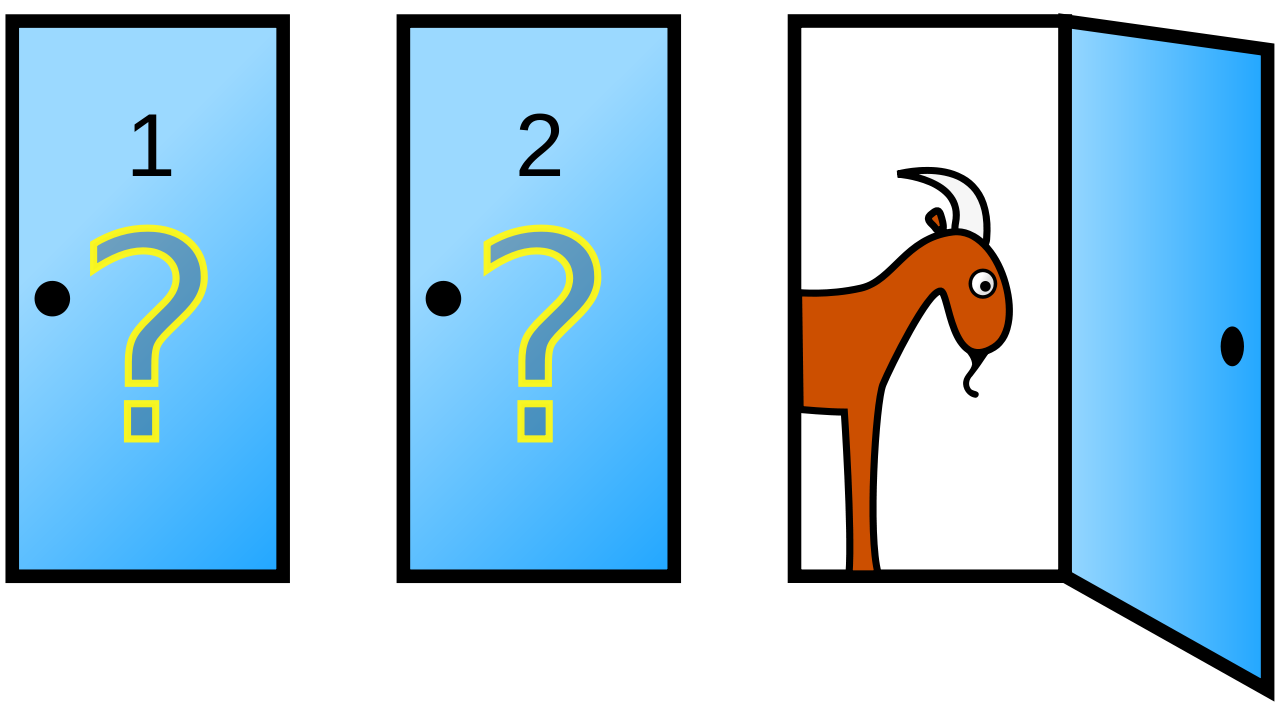
\includegraphics[width=8cm]{chapters/montyhall.png}
    \caption{ภาพแสดงการเปิดประตูไปเจอแพะ}
    \label{fig:montyhall}
\end{figure}

\begin{exercise}
หากคุณเป็นผู้เข้าร่วมเกมโชว์ และอยากได้รางวัลเป็นรถยนต์ คุณจะเลือกที่จะสลับประตูที่เปิดหลังพิธีกรเปิดประตูที่เป็นแพะหรือไม่? เพราะอะไร? และการเลือกสลับนี้มีผลต่อความน่าจะเป็นของการได้รางวัลเป็นรถยนต์หรือไม่ อย่างไร? จงอธิบาย
\end{exercise}

\section{Closest Pair of Points}

ปัญหาคลาสสิกปัญหาหนึ่งที่เป็นที่นิยมคือปัญหาคู่ของจุดที่ใกล้กันมากที่สุด (Closest pair of points) ก่อนจะไปถึงปัญหานั้น เราจะพิจารณาปัญหาที่ง่ายกว่านั้นก่อน

\begin{definition}
ให้สัญลักษณ์ $\delta(S)$ แทนระยะห่างของจุดที่ใกล้กันมากที่สุดใน $S$ (กล่าวได้ว่า $\delta \colon \R \times \R \to \R$ เป็นฟังก์ชัน)
\end{definition}

\begin{exercise}
ให้ $N \in \N$ กำหนดจุด $N$ จุดบนระนาบสองมิติ ในอาเรย์ $S$ และค่า $d$ มาให้ ให้ออกแบบอัลกอริทึมที่ตรวจสอบระหว่าง $\delta(S) > d$, $\delta(S) < d$ หรือ $\delta(S) = d$ ได้ในเวลา $O(N)$ (คำใบ้: ตารางกริดบนระนาบ)
\end{exercise}

พิจารณาอัลกอริทึมต่อไปนี้ ทำการสุ่มตำแหน่ง (shuffle) บน $S$ แล้วให้ $r_i := \delta(\{S_1, \dots, S_i\})$ จะได้ $r_1, r_2, \dots, r_N \in \R$ แล้วค่อย ๆ ดำเนินการคำนวณ $r_i$ โดยเริ่มจาก $r_1 = \infty$ แล้วค่อย ๆ ใส่จุดลงไปแล้วตรวจสอบว่า $r_i < r_{i-1}$ หรือไม่ หาก $r_i < r_{i-1}$ ทำการคำนวณหาค่า $r_i$ โดยหา $r_i = \min\{||S_i - S_j|| \colon j != i\}$ ใน $O(N)$

อัลกอริทึมข้างต้นจะใช้เวลา $O(kN)$ เมื่อ $k$ แทนจำนวนครั้งที่ $r_i < r_{i-1}$

เมื่อพิจารณาอย่างละเอียด จะกล่าวได้ว่าเวลารวมที่ใช้จะเป็นสัดส่วนกับ
\[
R = 1 + \sum_{i=2}^N (1 + i X_i)
\]
เมื่อ $X_i$ เป็นตัวแปรสุ่ม ที่หาก $r_i < r_{i-1}$ แล้วจะมีค่าเป็น $1$ มิฉะนั้นจะมีค่าเป็น $0$

\begin{exercise}
จงพิสูจน์ว่า $\Pr(X_i = 1) \leq \frac{2}{i}$ สำหรับทุก $i \in \{2, \dots, N\}$
\end{exercise}

\begin{exercise}
จงพิสูจน์ว่า $\mathbb{E}[R] \leq 3n$ และสรุปผล
\end{exercise}

\section{Bloom Filter}

โครงสร้างข้อมูลแบบหนึ่งมีชื่อว่า Bloom Filter โดยสามารถทำหน้าที่ได้ดังนี้
\begin{itemize}[nosep]
    \item ใส่ค่า $x$ ลงใน Bloom Filter
    \item ตรวจสอบว่ามีค่า $x$ อยู่ใน Bloom Filter หรือไม่
\end{itemize}

โดย Bloom Filter นั้น ข้อเสียคือเวลาตรวจสอบมีโอกาสผิดพลาดแบบ false positive (ตอบว่ามีทั้ง ๆ ที่ไม่มี) ได้ แต่ว่าจะไม่มีทางตอบว่าไม่มีทั้ง ๆ ที่มี ส่วนข้อดีคือเป็นโครงสร้างที่สร้างมาเพื่อประหยัดพื้นที่

หลักการทำงานของ Bloom Filter คือ หากเราทราบว่าจะมีการใส่ค่าทั้งหมด $n$ ค่า และเราต้องการเตรียม Bloom Filter ขนาด $m$ บิต เราจะสร้างแฮชฟังก์ชันที่แตกต่างกัน $k$ ฟังก์ชันที่ส่งผลลัพธ์อย่างสุ่ม

โดยเริ่มต้น เราจะปรับให้ทุกบิตของ Bloom Filter เป็นศูนย์ก่อน ต่อมา สมมติแฮชฟังก์ชันชื่อ $h_1, h_2, \dots, h_k$ เมื่อเราต้องการใส่ค่า $x$ ลงไป เราจะทำการคำนวณ $b_1 = h_1(x), b_2 = h_2(x), \dots, b_k = h_k(x)$ แล้วปรับค่าช่องที่ $b_1, b_2, \dots, b_k$ บน Bloom Filter ให้เป็นหนึ่งให้หมด

\begin{figure}[htbp]
    \centering
    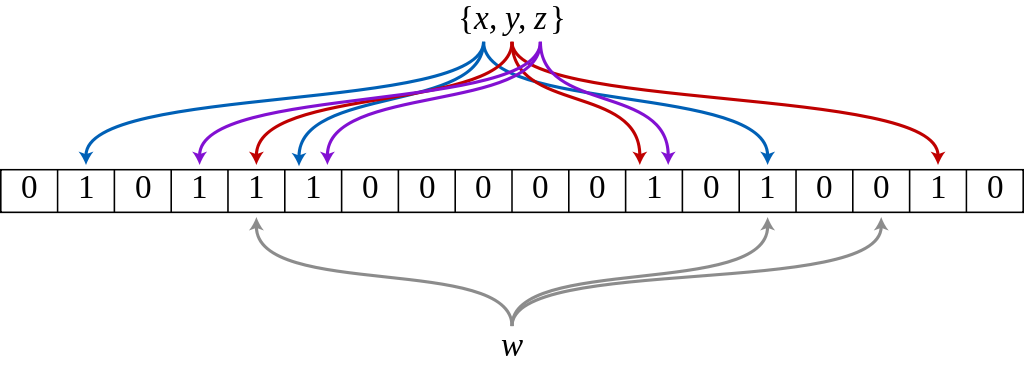
\includegraphics[width=10cm]{chapters/bloomfilter.png}
    \caption{รูปแสดงการทำงานของ Bloom Filter}
    \label{fig:bloom_filter}
\end{figure}

เมื่อมีคำถามว่ามี $x$ อยู่ในนี้หรือไม่ เราก็ทำการคำนวณ $b_1 = h_1(x), b_2 = h_2(x), \dots, b_k = h_k(x)$ เหมือนเดิม แล้วตรวจสอบว่าช่องที่ $b_1, b_2, \dots, b_k$ บน Bloom Filter นั้นเป็นหนึ่งทั้งหมดหรือไม่ หากมีช่องใดช่องหนึ่งไม่เป็นหนึ่ง เราสรุปได้ทันทีว่า $x$ ไม่อยู่ในนี้ แต่หากทุกช่องเป็น $1$ เราสรุปอะไรไม่ได้ จึงตอบได้ว่ามีความเป็นไปได้สูงที่ $x$ จะอยู่ในนี้

สมมติให้แฮชฟังก์ชันคืนค่าโดยสุ่มอย่างเท่าเทียบ (หมายถึงความน่าจะเป็นที่ $h(x) = i$ นั้นเท่ากันหมดสำหรับทุก $i$ จากทั้ง $m$ ช่อง) แสดงว่า ความน่าจะเป็นที่ $h(x)$ จะเท่ากับค่าค่าหนึ่ง มีค่าเท่ากับ $\frac{1}{m}$ 

\begin{exercise}
จงพิสูจน์ว่า หากแฮชฟังก์ชันไม่ค่อยจะเกิดการแทรกซ้อนกัน (ให้คิดเสียว่าแฮชฟังก์ชันแต่ละตัวไม่เกี่ยวข้องกัน) และ $m$ มีค่ามาก จงพิสูจน์ว่าความน่าจะเป็นที่บิตบิตหนึ่งจะยังเป็นศูนย์ หลังจากใส่ของลงไปไม่ซำ้กัน $n$ ชิ้น จะมีค่าประมาณ $e^\frac{-kn}{m}$

(คำใบ้: เนื่องจาก $\lim\limits_{m \to \infty} \left(1-\frac{1}{m}\right)^m = e$ เราจึงสามารถประมาณค่า $\left(1-\frac{1}{m}\right)^m \approx e$ ได้)
\end{exercise}

\begin{exercise}
คราวนี้ เมื่อพิจารณาการทดสอบว่า $x$ อยู่ใน Bloom Filter หรือไม่ จงพิสูจน์ว่าความน่าจะเป็นที่จะตอบผิด (ไม่อยู่แต่ตอบว่าอยู่) มีค่าประมาณ
\[
\varepsilon = (1-e^\frac{-kn}{m})^k
\]
\end{exercise}

\begin{exercise}
จงพิสูจน์ว่า หากทราบค่า $m$ และ $n$ ล่วงหน้าแล้ว ค่า $k$ ที่ดีที่สุดจะมีค่าใกล้เคียงกับ $\frac{m}{n} \ln(2)$
\end{exercise}

\begin{exercise}
หาก $k = \frac{m}{n} \ln(2)$ และ $n = 1\,000\,000$ จะต้องใช้หน่วยความจำกี่บิต (กล่าวคือจงหาค่าของ $m$ ที่น้อยที่สุด) เพื่อที่จะมั่นใจได้ว่าความน่าจะเป็นที่จะตอบถูกมีค่าอย่างน้อย $95\%$
\end{exercise}
\chapter{Basic Dynamic Programming}

\section{Travelling Salesman Problem}

ปัญหา TSP เป็นปัญหาที่ถามว่า หากกำหนดกราฟไม่ระบุทิศทางแต่ถ่วงนำ้หนักมาให้กราฟหนึ่ง คือ $G = (V, E)$ ประกอบด้วย $N$ จุดยอด และ $M$ เส้นเชื่อม เซลล์แมนต้องการเดินทางไปให้ครบทุกจุดยอด จะเดินทางอย่างไรให้ผลรวมนำ้หนักบนการเดินทางนั้นมีค่าน้อยที่สุด

กล่าวคือ หากให้ $dist \colon V \times V \to \R$ แทนระยะทางที่สั้นที่สุดจากสองจุดบนกราฟ และให้ $\phi \colon V \to V$ เป็นฟังก์ชันหนึ่งต่อหนึ่งทั่วถึงแล้ว ปัญหา TSP ต้องการหาค่า
\[
\min_{\phi} \sum_{i=1}^{N-1} dist(\phi(i), \phi(i+1))
\]

เนื่องจาก $dist$ นั้นคำนวณมาก่อนได้ (มันคือปัญหา APSP: All-Pairs Shortest Path) ในเวลาเพียง $O(N^3)$ ส่วนใหญ่จึงให้ $M = \frac{N(N-1)}{2}$ และ $G$ เป็นกราฟบริบูรณ์ไปเลย แล้วทำการตอบปัญหา TSP ในรูปแบบ
\[
\min_{\phi} \sum_{i=1}^{N-1} D_{\phi(i), \phi(i+1)}
\]
แทน เมื่อ $D$ เป็นตารางสองมิติขนาด $N \times N$

\begin{exercise}
จงออกแบบอัลกอริทึมที่แก้ปัญหา TSP ได้ใน $O(2^N N^2)$
\end{exercise}

นอกจากนี้ยังมีปัญหา TSP ที่ปรับให้มีเงื่อนไขพิเศษ คือให้จุดแต่ละจุดอยู่บนระนาบสองมิติและใช้ระยะทางแบบยูคลิด (Euclidean Distance) แล้วบังคับว่าจะต้องเดินทางจากจุดซ้ายสุด ไปยังจุดขวาสุดก่อน แล้วค่อยย้อนกลับมา (ไม่สามารถเดินซ้ายสลับขวามั่ว ๆ ได้) เรียกปัญหานี้ว่า Bitonic TSP

\begin{exercise}
จงออกแบบอัลกอริทึมที่แก้ปัญหา Bitonic TSP ได้ใน $O(N^2)$
\end{exercise}

\begin{bonus}
มีอัลกอริทึมที่แก้ปัญหา Bitonic TSP ที่ดีกว่า $O(N^2)$ หรือไม่?
\end{bonus}

\section{Ternary Tree Traversal}
\label{ipst:o59_oct_c1_ternary}

ต้นไม้ตรีภาค คือต้นไม้ที่ปมแต่ละปมนั้นอาจจะมีลูกได้สามปม ได้แก่ ลูกซ้าย ลูกกลาง และ ลูกขวา กำหนดให้การหา preorder traversal และ inorder traversal ของปมในต้นไม้ต้นนี้เขียนเป็นรหัสเทียมได้ดังนี้ โดยให้ \texttt{left\_child(x)}, \texttt{center\_child(x)} และ \texttt{right\_child(x)} คือลูกซ้าย ลูกกลาง และ ลูกขวา ของปม \texttt{x} ตามลำดับ

\noindent\begin{minipage}{.48\textwidth}
\begin{lstlisting}[caption=Preorder]{Preorder}
preorder(node x) {
  if (x == NULL) return
  print(value(x))
  preorder(left_child(x))
  preorder(center_child(x))
  preorder(right_child(x))
}
\end{lstlisting}
\end{minipage}\hfill
\begin{minipage}{.48\textwidth}
\begin{lstlisting}[caption=Inorder]{Inorder}
inorder(node x) {
  if (x == NULL) return
  inorder(left_child(x))
  print(value(x))
  inorder(center_child(x))
  inorder(right_child(x))
}
\end{lstlisting}
\end{minipage}

เรามีต้นไม้ตรีภาคขนาด $n$ ปมอยู่ต้นหนึ่ง ซึ่งแต่ละปมนั้นกำกับด้วยจำนวนเต็มหนึ่งตัว ซึ่งมีค่าตั้งแต่ $0$ ถึง $n-1$  โดยที่แต่ละปมไม่ซำ้กันเลย จากข้อมูลผลการทำงานของ preorder traversal และ inorder traversal ที่ปมรากของต้นไม้ต้นนี้ จงคำนวณว่ามีต้นไม้กี่ต้น (รวมทั้งต้นไม้ของเรานี้ด้วย) ที่มีผลการทำงาน preorder และ inorder ตรงกับที่กำหนดให้

เนื่องจากคำตอบอาจมีค่าสูงมาก ให้ตอบเฉพาะจำนวนหารเอาเศษด้วย $10^9+7$

(โจทย์จากข้อ \texttt{o59\_oct\_c1\_ternary})

\begin{exercise}
จงพิสูจน์ว่า หากจำนวนเต็มตัวแรกของ preorder traversal มีค่าเท่ากับจำนวนเต็มตัวสุดท้ายของ inorder traversal แล้วรากของต้นไม้นี้จะไม่มีลูกตรงกลางและลูกทางขวา
\end{exercise}

\begin{exercise}
จงพิสูจน์ว่า หากจำนวนเต็มตัวแรกของ preorder traversal มีค่าเท่ากับจำนวนเต็มตัวแรกของ inorder traversal แล้วรากของต้นไม้นี้จะไม่มีลูกทางซ้าย
\end{exercise}

\begin{exercise}
จงออกแบบอัลกอริทึมในการแก้ปัญหาข้อนี้ภายในเวลา $O(N^4)$ และใช้ความจำ $O(N^3)$
\end{exercise}

\begin{bonus}
มีวิธีที่เร็วกว่า $O(N^4)$ หรือใช้ความจำที่น้อยกว่า $O(N^3)$ หรือไม่?
\end{bonus}

\section{Incantation}
\label{ipst:o60_oct_c2_incantation}

จอมเวทย์คนหนึ่งจะร่ายมนต์ มนต์ประกอบด้วยคำพูดติดกัน $n$ พยางค์ พยางค์แต่ละพยางค์เป็นไปได้สองแบบคือ \texttt{IN} และ \texttt{ORT} ตัวอย่างมนต์ที่ประกอบด้วยสามพยางค์คือ \texttt{IN ORT IN} หรือ \texttt{ORT ORT ORT} เป็นต้น ความแข็งแกร่งของมนต์นั้นขึ้นอยู่กับลำดับของพยางค์ต่าง ๆ ที่ปรากฎอยู่ในมนต์

จองเวทย์ศึกษาจนรู้ว่า ความแข็งแกร่งของมนต์นั้นสามารถคำนวณได้จากตารางความแข็งแกร่งของคำใดๆ ก็ตามที่มีความยาวเท่ากับ $k$ กล่าวคือ คำที่มีความยาว $k$ พยางค์ใด ๆ จะมีค่าความแข็งแกร่งอยู่ค่าหนึ่ง ความแข็งแกร่งของมนต์จะเท่ากับผลรวมของจำนวนครั้งที่คำความยาว $k$ นั้นปรากฎขึ้นคูณด้วยค่าความแข็งแกร่งของคำนั้นจากตารางที่กำหนดให้ สำหรับคำความยาว $k$ ทุกคำที่เป็นไปได้นั่นเอง

ตัวอย่างเช่น เมื่อ $n = 5$ และ $k = 2$ มนต์ \texttt{IN ORT IN ORT ORT} จะมีค่าความแข็งแกร่งเท่ากับ $(\text{ความแข็งแกร่งของ } \texttt{IN ORT} \cdot 2) + (\text{ความแข็งแกร่งของ } \texttt{ORT IN} \cdot 1) + (\text{ความแข็งแกร่งของ } \texttt{ORT ORT} \cdot 1)$ เป็นต้น

จากตารางความแข็งแกร่งของคำความยาว $k$ พยางค์ทั้งหมดที่กำหนดให้ จงหาว่ามนต์ที่แข็งแกร่งที่สุดที่เป็นไปได้นั้นมีค่าความแข็งแกร่งเท่าไร

(โจทย์จากข้อ \texttt{o60\_oct\_c2\_incantation})

\begin{exercise}
จงออกแบบอัลกอริทึมที่แก้ปัญหานี้ได้ใน $O(nk)$
\end{exercise}

\begin{exercise}
จงออกแบบอัลกอริทึมที่แก้ปัญหานี้ได้ใน $O(8^k \log n)$
\end{exercise}

\begin{bonus}
มีวิธีที่ดีกว่านี้อีกหรือไม่?
\end{bonus}
\chapter{Graph algorithms + graph theory}

\section{Black-White Graph Coloring}

ในส่วนนี้จะพิจารณาเฉพาะกราฟไม่ระบุทิศทางที่ไม่มี self-loop (กล่าวคือไม่มีจุดยอดใดมีเส้นเชื่อมกับตัวเอง) เราจะทำการศึกษาวิธีการระบายสีกราฟที่สอดคล้องกับเงื่อนไขต่อไปนี้
\begin{enumerate}[nosep]
    \item จุดยอดทุกจุดยอดจะมีสีกำหนดอยู่ เป็นอย่างใดอย่างหนึ่งระหว่างสีขาวและสีดำ
    \item สำหรับจุดยอด $u$ และ $v$ ที่อยู่ติดกัน (กล่าวคือ มีเส้นเชื่อม $\{u, v\} \in E$) สีของ $u$ กับ $v$ นั้นต่างกัน
\end{enumerate}

\begin{exercise}
จงพิสูจน์ว่าในกราฟเส้นตรง (กล่าวคือ $G = (V, E)$ เมื่อ $V = \{1, \dots, N\}$ และ $E = \{\{i, i+1\} \colon i \in \{1, \dots, N-1\}\}$ สำหรับจำนวนเต็มบวก $N$ ใด ๆ) จะมีวิธีการระบายสีกราฟตามเงื่อนไขข้างต้นอยู่ $2$ วิธี
\end{exercise}

\begin{exercise}
จงพิสูจน์ว่าหากกราฟไม่ใช่ Bipartite Graph แล้วจะไม่มีวิธีการระบายสีตามเงื่อนไขดังกล่าว (คำใบ้: พิสูจน์โดยแย้งสลับที่)
\end{exercise}

\begin{exercise}
จงพิสูจน์ว่าหากกราฟเป็น Bipartite Graph ที่เชื่อมต่อกัน (connected) แล้วจะมีวิธีการระบายสีตามเงื่อนไขอยู่ $2$ วิธี
\end{exercise}

\begin{exercise}
จงพิสูจน์ว่าหากกราฟ $G$ เกิดจากการนำกราฟ $G_1$ มารวม (union) กับกราฟ $G_2$ และกราฟ $G_1$ และ $G_2$ มีวิธีการระบายสีอยู่ $c_1$ แบบและ $c_2$ แบบตามลำดับ แล้ววิธีการระบายสีบนกราฟ $G$ จะมีอยู่ทั้งหมด $c_1 \cdot c_2$ แบบ
\end{exercise}

\begin{exercise}
จงพิสูจน์ข้อสรุป ว่าใน Bipartite Graph ที่ประกอบด้วย $C$ ส่วนเชื่อมต่อกัน (connected component) จะมีวิธีการระบายสีทั้งหมด $2^C$ แบบ
\end{exercise}

\section{DFS and Topological Sort}

ในส่วนนี้จะใช้ $N$ แทนจำนวนจุดยอดและ $M$ แทนจำนวนเส้นเชื่อม

นอกจาก Kahn's Algorithm ที่ใช้ในการหา Topological Ordering บน DAG ใน $O(N+M)$ ได้แล้ว เราจะพิจารณาอัลกอริทึมที่ค่อนข้างง่ายอีกอัลกอริทึมหนึ่ง ตังต่อไปนี้

\begin{enumerate}[nosep]
    \item สร้างสแตคเปล่า ชื่อ $S$
    \item สำหรับแต่ละจุดยอดในกราฟ ให้ทำการ DFS จากจุดยอดนั้น จนกว่าจะหมดกราฟโดยเมื่อทำ DFS เสร็จจะทำการใส่ของลงในสแตค
    \item ค่อย ๆ นำของออกจาก $S$ จากบนสุดของสแตคจนถึงล่างสุด ลำดับของจุดยอดที่นำออกมา จะสอดคล้องกับลำดับ Topological Order
\end{enumerate}

หรือพิจารณาโค้ดตัวอย่างดังต่อไปนี้

\begin{lstlisting}
std::vector<int> G[N+1]; // adjacency list
std::stack<int> S;
bool found[N+1]; // initially set to false
void dfs(int u){
    if(found[u]) return;
    for(int v : G[u]){
        dfs(v);
    }
    S.push(u);
}
\end{lstlisting}

และเมื่อได้กราฟมาแล้วจะทำการรันดังต่อไปนี้

\begin{lstlisting}
for(int u = 1; u <= N; u++){
    dfs(u);
}
while(!S.empty()){
    std::cout << S.top() << std::endl;
    S.pop();
}
\end{lstlisting}

\begin{exercise}
จงพิสูจน์ว่าอัลกอริทึมดังกล่าวให้ผลลัพธ์ออกมาเป็น Topological Order และใช้เวลาใน $O(M+N)$
\end{exercise}

\begin{bonus}
มีอัลกอริทึมที่สามารถหา Topological Order ที่ Lexicographical Order น้อยสุดที่เป็นไปได้สำหรับทุก Topological Order ที่เป็นไปได้หรือไม่ในเวลา $O(M+N)$
\end{bonus}

\section{Sun Graphs}

\begin{exercise}
สำหรับกราฟที่เชื่อมต่อกันที่เป็น simple graph (ไม่มีลูปวนซำ้ตัวเอง และไม่มีเส้นเชื่อมขนาน) ที่มีจำนวนจุดยอดเท่ากับจำนวนเส้นเชื่อม จงพิสูจน์ว่ากราฟนี้จะมีวัฏจักร (cycle) อยู่ $1$ อันพอดี และเมื่อลบวัฏจักรนี้ทิ้งออกไปจะเหลือเป็นป่า (forest) (หมายถึง กราฟที่ประกอบด้วยต้นไม้หลายต้น หรือต้นเดียว หรือไม่มีต้นไม้เลยก็เป็นได้)

ในส่วนนี้จะขอเรียกกราฟประเภทนี้ว่ากราฟดวงอาทิตย์ (ไม่ใช่ชื่อเรียกทางการ; ไม่สามารถใช้นอกขอบเขตนี้ได้)
\end{exercise}

\begin{exercise}
จงพิสูจน์ว่าสำหรับกราฟที่เป็น simple graph แต่อาจไม่เชื่อมต่อกันนั้น เราสามารถแบ่งกราฟนี้เป็นผลรวม (union) ของกราฟดวงอาทิตย์หลาย ๆ กราฟได้
\end{exercise}

\section{Smallest Fibonacci-covered-difference Set}
\label{imo:2020slc4}

นิยามจำนวนฟิโบนัชชี $F_0, F_1, \dots$ จาก $F_0 = 0$, $F_1 = 1$ และ $F_{n+1} = F_{n} + F_{n-1}$ สำหรับทุกจำนวนเต็ม $n \geq 1$ ให้จำนวนเต็ม $n \geq 2$ จงหาขนาดที่เล็กที่สุดที่เป็นไปได้ของเซต $S$ ที่สำหรับทุก $k = 2, 3, \dots, n$ จะมีบาง $x, y \in S$ ที่ $x - y = F_k$

(โจทย์จาก IMO 2020 Shortlist ข้อ C4.)

สำหรับเซต $S \subseteq \Z$ ใด ๆ ที่สอดคล้องกับเงื่อนไข เราจะทำการสร้างกราฟดังนี้ ให้ $G$ เป็นกราฟไม่ระบุทิศทางถ่วงนำ้หนัก โดยมีเส้นเชื่อมเป็นเซตเดียวกับ $S$ และสำหรับทุกจำนวนเต็ม $1 \leq k \leq \lceil \frac{n}{2} \rceil$ เลือก $x, y \in S$  ที่ $x - y = F_{2k+1}$ แล้วเติมเส้นเชื่อม $\{x, y\}$ ลงไปในกราฟ

\begin{exercise}
จงพิสูจน์ว่าสำหรับแต่ละจำนวนเต็ม $1 \leq k \leq \lceil \frac{n}{2} \rceil$ จะสามารถเลือก $x, y \in S$ ที่ $x - y = F_{2k+1}$ ได้เสมอ
\end{exercise}

\begin{exercise}
จงพิสูจน์ว่ากราฟดังกล่าวไม่มีวัฏจักร (cycle)
\end{exercise}

\begin{exercise}
จงพิสูจน์ว่าสำหรับทุกเซต $S \subseteq \Z$ ที่สอดคล้องกับเงื่อนไข จะได้ว่า $|S| \geq \lceil \frac{n}{2} \rceil + 1$
\end{exercise}

\begin{exercise}
จงพิสูจน์ว่ามีเซต $S$ ที่สอดคล้องกับเงื่อนไขที่ $|S| = \lceil \frac{n}{2} \rceil + 1$ และสรุปผล
\end{exercise}
\chapter{Greedy \& MST}

\newcommand{\bene}{\mathsf{B}}
\newcommand{\mb}{\mathsf{MB}}
\section{Consumer Problem}

ในการศึกษาเศรษฐศาสตร์ ซึ่งว่าด้วยการจัดสรรทรัพยากรที่มีอยู่อย่างจำกัดให้กับความต้องการที่มีอยู่อย่างไม่จำกัด ปัญหาหนึ่งที่เป็นปัญหาพื้นฐานและสำคัญ คือปัญหาของผู้บริโภค

สมมติผู้บริโภคมีเงินอยู่จำกัด (เรียกว่า $B$ หน่วย) และต้องการซื้อสินค้าสองชนิด เรียกว่าชนิด \textbf{ก} กับชนิด \textbf{ข} โดยที่ผู้บริโภคจะนิยามฟังก์ชันผลประโยชน์ ตามตารางดังนี้

\begin{center}
\begin{tabular}{|c|c|c|}
\hline
จำนวน (ชิ้น) & ผลประโยชน์ที่ได้จากการซื้อ \textbf{ก} (หน่วย) & ผลประโยชน์ที่ได้จากการซื้อ \textbf{ข} (หน่วย) \\
\hline
1 & 100 & 160 \\
2 & 185 & 310 \\
3 & 260 & 410 \\
4 & 325 & 490 \\
5 & 385 & 520 \\
6 & 435 & 530 \\
7 & 480 & 533 \\
8 & 520 & 535 \\
\hline
\end{tabular}
\end{center}

\begin{exercise}
สมมติว่า สินค้าชนิด \textbf{ก} ราคา 25 บาท และสินค้าชนิด \textbf{ข} ราคา 50 บาท หากผู้บริโภคมีงบ 300 บาท จะมีโอกาสซื้อผลลัพธ์ออกมาได้กี่แบบ
\end{exercise}

\begin{exercise}
สมมติว่า สินค้าชนิด \textbf{ก} ราคา 25 บาท และสินค้าชนิด \textbf{ข} ราคา 50 บาท หากผู้บริโภคมีงบ 300 บาท จะซื้อชนิด \textbf{ก} กี่ชิ้น และชนิด \textbf{ข} กี่ชิ้น เพื่อให้ได้ผลประโยชน์รวมสูงสุด
\end{exercise}

พิจารณาอัลกอริทึมในการตัดสินใจซื้อสินค้า ดังต่อไปนี้
\begin{enumerate}[nosep]
    \item คำนวณผลประโยชน์ส่วนเพิ่ม (marginal benefit) โดยสำหรับสินค้าแต่ละชนิดนั้นผลประโยชน์ส่วนเพิ่มจากการซื้อสินค้าไป $k$ ชิ้น คือผลประโยชน์ที่ได้รับมาเพิ่มขึ้นจากที่มีอยู่ $k-1$ ชิ้น (พิจารณาตารางหลังจากนี้)
    \item คำนวณผลประโยชน์ส่วนเพิ่มต่อเงินที่จะต้องเสียไป (หน่วยต่อบาท) โดยสามารถพิจารณาได้ในตารางหลังจากนี้
    \item จากที่มีเงินอยู่ $B$ บาท และยังไม่ได้ซื้อสินค้าอะไรเลย ค่อย ๆ เลือกซื้อสินค้าที่ \textbf{ผลประโยชน์ส่วนเพิ่มต่อเงินที่ต้องเสียไป} มีค่ามากกว่า
    \item ทำซำ้ จนกว่าเงินจะหมดงบ
\end{enumerate}

\begin{center}
\begin{tabular}{|c|c|c|c|c|c|c|}
\hline
$n$ & $\bene_\text{ก}(n)$ & $\mb_\text{ก}(n)$ & $\mb_\text{ก}(n)/p_\text{ก}$ & $\bene_\text{ข}(n)$ & $\mb_\text{ข}(n)$ & $\mb_\text{ข}(n)/p_\text{ข}$ \\
\hline
1 & 100 & 100 & 4 & 160 & 160 & 3.2 \\
2 & 185 & 85 & 3.4 & 310 & 150 & 3 \\
3 & 260 & 75 & 3 & 410 & 100 & 2 \\
4 & 325 & 65 & 2.6 & 490 & 80 & 1.6 \\
5 & 385 & 60 & 2.4 & 520 & 30 & 0.6 \\
6 & 435 & 50 & 2 & 530 & 10 & 0.2 \\
7 & 480 & 45 & 1.8 & 533 & 3 & 0.06 \\
8 & 520 & 40 & 1.6 & 535 & 2 & 0.04 \\
\hline
\end{tabular}
\end{center}

เมื่อ
\begin{itemize}[nosep]
    \item $n$ แทนจำนวน
    \item $\bene_x(n)$ แทนผลประโยชน์จากการซื้อสินค้าชนิด $x$ ไป $n$ ชิ้น
    \item $\mb_x(n)$ แทนผลประโยชน์ส่วนเพิ่มจากการซื้อสินค้าชนิด $x$ จาก $n-1$ เป็น $n$ ชิ้น
    \item $\frac{\mb_x(n)}{p_x}$ แทนผลประโยชน์ส่วนเพิ่มต่อเงินที่ต้องเสียไป (ในที่นี้คือราคาสินค้า) 
\end{itemize}

จากกรณีข้างต้น อัลกอริทึมดังกล่าวจะซื้อสินค้าชนิด \textbf{ก} จำนวน 6 ชิ้น และชนิด \textbf{ข} จำนวน 3 ชิ้น

\begin{exercise}
พิจารณากรณีทั่วไป หากรับประกันว่าสำหรับทุกจำนวนเต็มบวก $n$, $0 \leq \mb_x(n+1) \leq \mb_x(n)$ เมื่อ $x \in \{\text{ก}, \text{ข}\}$ แล้วจงพิสูจน์ว่าอัลกอริทึมดังกล่าวทำงานถูกต้อง กล่าวคือผลลัพธ์ของอัลกอริทึมดังกล่าวจะให้ผลรวมของผลประโยชน์ของการซื้อสินค้าทั้งสองชนิดออกมาสูงที่สุดเท่าที่จะเป็นไปได้
\end{exercise}

\begin{exercise}
อัลกอริทึมนี้จะยังถูกหรือไม่หากขยายให้มีสินค้ามากกว่าสองชนิด
\end{exercise}

\begin{exercise}
อัลกอริทึมข้างต้นใช้เวลา $O(N)$ ในการคำนวณ เมื่อ $N$ แทนจำนวนสินค้ามากที่สุดที่ซื้อได้ จงออกแบบอัลกอริทึมที่ทำงานได้เหมือนกันแต่ใช้เวลาเพียง $O(\log N)$
\end{exercise}

\begin{bonus}
หาก $\bene_x$ ไม่ใช่แค่ฟังก์ชันที่รับจำนวนเต็มเท่านั้นแต่ขยายเป็นจำนวนจริง และรับประกันว่า $\bene_x$ เป็นฟังก์ชันต่อเนื่องและหาอนุพันธ์ได้สองครั้ง และรับประกันว่า $\bene_x''(t) \geq 0$ สำหรับทุกจำนวนจริง $t > 0$ จงพิสูจน์ว่าเราสามารถใช้อัลกอริทึมข้างต้นแก้ปัญหานี้ (โดยการประมาณค่า) ได้
\end{bonus}

\section{Minimax Path}

ให้กราฟไม่ระบุทิศทางถ่วงนำ้หนักมากราฟหนึ่ง ประกอบด้วย $N$ จุดยอดและ $M$ เส้นเชื่อม ประกอบกับคำถาม $Q$ คำถาม แต่ละคำถามถามว่า หากต้องการเดินทางจากจุดยอด $u$ ไปยังจุดยอด $v$ โดยให้ค่ามากสุดของเส้นเชื่อมแต่ละเส้นที่ใช้เดินทางนั้นออกมามีค่าน้อยที่สุดเท่าที่เป็นไปได้

\begin{exercise}
หาก $Q = 1$ จงออกแบบอัลกอริทึมที่แก้ปัญหานี้ได้ใน $O(M \log N)$
\end{exercise}

\begin{exercise}
จงพิสูจน์ว่าสำหรับทุกคำถาม หากพิจารณาเฉพาะ path จาก $u$ ไปหา $v$ บน MST เท่านั้นจะยังคงให้คำตอบที่ถูกต้องอยู่
\end{exercise}

\begin{exercise}
สำหรับกราฟประเภทต้นไม้ (คนละกราฟกับกราฟหลักของข้อนี้) ที่ประกอบด้วย $N'$ จุดยอด จงออกแบบอัลกอริทึมที่สามารถหาเส้นเชื่อมที่มีค่ามากสุดระหว่างจุดยอด $u$ กับ $v$ ใด ๆ ในกราฟนี้ ภายในเวลา $O(\log N')$ ต่อคำถาม และให้เวลาเตรียมการภายในเวลา $O(N' \log N')$
\end{exercise}

\begin{exercise}
จงออกแบบอัลกอริทึมที่แก้ปัญหานี้ได้ใน $O(M \log N + Q \log N)$
\end{exercise}
\chapter{Shortest Paths}

\section{Dijkstra's Algorithm Variants}

\begin{exercise}
สำหรับปัญหาการหาเส้นทางที่สั้นที่สุดระหว่างจุดยอดสองจุดในกราฟไม่ระบุทิศทางถ่วงนำ้หนัก ที่ประกอบด้วย $N$ จุดยอด และ $M$ เส้นเชื่อม เรารู้ว่า Dijkstra's Algorithm ทำงานได้ใน $O(M \log N)$ อย่างไรก็ตาม สำหรับกราฟที่หนาแน่น (dense) มาก จะทำให้ $M \in \Theta(N^2)$ ทำให้อัลกอริทึมดังกล่าวทำงานใน $O(N^2 \log N)$ จงออกแบบอัลกอรทึมที่ดีกว่านี้ ที่ทำงานได้ใน $O(N^2)$
\end{exercise}

\begin{exercise}
นอกจากนี้ สำหรับกราฟที่นำ้หนักเป็นจำนวนเต็มที่รับประกันว่าผลรวมนำ้หนักมีค่าไม่เกิน $W$ จงออกแบบอัลกอริทึมที่หาเส้นทางที่สั้นที่สุดได้ใน $O(MW)$
\end{exercise}

\section{Systems of Inequalities}

\begin{exercise}
กำหนดตัวแปรไม่ทราบค่า $n$ ตัว คือ $x_1, x_2, \dots, x_n$ โดยค่าของแต่ละตัวเป็นจำนวนเต็ม กำหนดระบบของอสมการทั้งหมด $m$ อสมการ ในรูปแบบ $x_i \leq x_j + k$ สำหรับบางจำนวนเต็ม $1 \leq i, j \leq n$ และ $k$ จงออกแบบอัลกอริทึมที่ตอบค่ามากสุดของ $x_n - x_1$ ที่สอดคล้องกับระบบอสมการนี้
\end{exercise}

\section{Legacy}
\label{codeforces:786B}

ก่อนจะเข้าสู่ปัญหาหลัก มีข้อสังเกตหนึ่งมาให้พิจารณาก่อน

\begin{exercise}
ให้ $A, B$ เป็นเซตของจุดยอดที่ $A \cap B = \emptyset$ สำหรับกราฟ $G = (V, E)$ โดย $V = A \cup B$ และ $E = A \times B$ พิจารณากราฟ $G' = (V', E')$ โดย $V' = A \cup B \cup \{c^*\}$ เมื่อ $c^* \notin A, B$ เป็นจุดยอดพิเศษ และนิยาม $E' = A \times c^* \cup c^* \times B$

จงพิสูจน์ว่าสำหรับทุก $u, v \in V$, $d'(u, v) = 2d(u, v)$ โดย $d'(u, v)$ แทนระยะทางสั้นสุดจาก $u$ ไปยัง $v$ บน $G'$ และ $d(u, v)$ แทนระยะทางสั้นสุดจาก $u$ ไปยัง $v$ บน $G$
\end{exercise}

มีกราฟระบุทิศทางถ่วงนำ้หนักอยู่กราฟหนึ่ง โดยระบุจุดยอดเป็นจุด $1, \dots, n$ สำหรับบางจำนวนเต็มบวก $n$ ตอนแรกยังไม่มีเส้นเชื่อมใด ๆ

ต่อมามีการก่อสร้างทั้งหมด 3 รูปแบบ ซึ่งจะทำให้เกิดเส้นเชื่อมบนกราฟ โดยแต่ละรูปแบบเป็นดังต่อไปนี้

\begin{enumerate}
    \item สร้างเส้นเชื่อมจากจุดยอด $v$ ไปหาจุดยอด $u$ ด้วยนำ้หนัก $w$
    \item สร้างเส้นเชื่อมจากจุดยอด $v$ ไปหาทุกจุดยอด $u$ ในช่วง $[l, r]$ ด้วยนำ้หนัก $w$
    \item สร้างเส้นเชื่อมจากทุกจุดยอด $u$ ในช่วง $[l, r]$ ไปหาจุดยอด $v$ ด้วยนำ้หนัก $w$
\end{enumerate}

ให้จุดยอด $s$ มา แทนจุดยอดเริ่มต้น จงหาระยะทางสั้นสุดจาก $s$ ไปยัง $1, \dots, n$ หากไปไม่ได้ให้ตอบ $-1$

\begin{exercise}
จงออกแบบอัลกอริทึมที่สามารถแก้ปัญหานี้ได้ใน $O(n \log^2 n)$ เมื่อจำนวนการก่อสร้างมีอยู่ $n$ ครั้ง
\end{exercise}

โจทย์จาก \url{https://codeforces.com/problemset/problem/786/B}

\chapter{Advanced Data Structures}

\section{RMQ versus LCA}

ในข้อนี้ให้ $N, Q$ เป็นจำนวนเต็มบวก

พิจารณาปัญหา RMQ ซึ่งกล่าวไว้ว่า มีอาเรย์ของจำนวนเต็ม $N$ ตัวและมีคำถาม $Q$ คำถาม แต่ละคำถาม ถามว่าระหว่างตัวที่ $l$ ถึง $r$ ตัวที่มีค่าน้อยที่สุดเป็นตัวที่เท่าใด

พิจารณาปัญหา LCA ซึ่งกล่าวไว้ว่า ให้ต้นไม้ระบุราก ประกอบด้วยจุดยอด $N$ จุดยอดและมีคำถาม $Q$ คำถาม แต่ละคำถาม ถามว่าจุดยอดที่เป็นบรรพบุรุษร่วมที่อยู่ตำแหน่งน้อยที่สุด (lowest common ancestor) ของ $u$ กับ $v$ คือจุดยอดใด

\begin{exercise}
อธิบายการทำงานของอัลกอริทึมที่ตอบปัญหา RMQ ได้ โดยเตรียมการ $O(N)$ และตอบคำถามแต่ละคำถามใน $O(\log N)$
\end{exercise}

\begin{exercise}
อธิบายการทำงานของอัลกอริทึมที่ตอบปัญหา LCA ได้ โดยเตรียมการ $O(N \log N)$ และตอบคำถามแต่ละคำถามใน $O(\log N)$
\end{exercise}

พิจารณาการแก้ปัญหา LCA ด้วยวิธีการดังต่อไปนี้

\begin{lstlisting}
std::vector<int> tour;
std::vector<int> children[N+1];
int start[N+1];
void dfs(int current, int parent, int depth){
    start[current] = tour.size();
    tour.push_back(depth);
    for(int child : children[current]){
        if(child == parent) continue;
        dfs(child, current, depth+1);
        tour.push_back(depth);
    }
}
\end{lstlisting}

\begin{exercise}
สังเกตว่า LCA ระหว่างจุดยอด \texttt{u} กับ \texttt{v} คือ RMQ ใน \texttt{tour} ระหว่างตัวที่ \texttt{start[u]} กับ \texttt{start[v]} จงพิสูจน์ว่า \texttt{tour} มีขนาดอยู่ใน $O(N)$ และพิสูจน์ว่าหากปัญหา RMQ มีวิธีแก้โดยการเตรียมการ $T_1(N)$ และตอบคำถามใน $T_2(N)$ แล้ว LCA จะสามารถแก้ได้โดยการเตรียมการใน $T_1(N) + O(N)$ และตอบคำถามใน $T_2(N) + O(1)$
\end{exercise}

ต่อมา พิจารณาโครงสร้างข้อมูล Cartesian Tree ซึ่งเป็นต้นไม้ทวิภาค ที่ทำบนอาเรย์ $A$ นิยามโดย

\begin{enumerate}
    \item สำหรับแต่ละจุดยอดใน Cartesian Tree นี้ จุดยอดที่เป็นลูกของจุดยอดปัจจุบัน จะมีค่ามากกว่าจุดยอดปัจจุบัน หรืออาจกล่าวได้ว่า parent ของแต่ละจุดยอดมีค่าน้อยกว่าจุดยอดนั้น ๆ
    \item หากทำการเดินทางบนต้นไม้แบบตามลำดับ (in-order traversal) แล้วจะได้ผลลัพธ์เป็นอาเรย์ $A$
\end{enumerate}

\begin{exercise}
จงแสดงว่าสำหรับอาเรย์ $A$ ที่ไม่มีสมาชิกซำ้กันเลยจะมี Cartesian Tree สำหรับ $A$ อยู่แบบเดียวเท่านั้น
\end{exercise}

% ต่อมา พิจารณาการแก้ปัญหา RMQ ด้วยวิธีการเตรียมการดังต่อไปนี้

% \begin{enumerate}
%     \item สำหรับ RMQ บนอาเรย์ $A$ สมมติ $A$ มีสมาชิกสองตัวที่มีค่าเท่ากัน กำหนดให้เรียงตามลำดับดัชนี (index) ว่าตัวใดมาก่อน เรียกอาเรย์ใหม่ว่า $A'$
%     \item สร้าง Cartesian Tree สำหรับ $A'$
% \end{enumerate}

% แล้วสำหรับคำถามแต่ละคำถามที่ถามหา RMQ บนช่วง $[l, r]$ ก็ให้ตอบคำถาม LCA บนจุดยอดที่แทนจำนวน $l$ และ $r$

\begin{exercise}
จงพิสูจน์ว่าหากปัญหา LCA มีวิธีแก้โดยการเตรียมการ $T_1(N)$ และตอบคำถามใน $T_2(N)$ แล้ว RMQ จะสามารถแก้ได้โดยการเตรียมการใน $T_1(N) + O(N)$ และตอบคำถามใน $T_2(N) + O(1)$
\end{exercise}

\section{Sparse Table}

\begin{exercise}
สำหรับข้อมูลอาเรย์ $[1, 8, 4, 2, 7, 5, 9, 6]$ จงวาด Sparse Table ที่สอดคล้องกับข้อมูลนี้ (สำหรับการหาค่าน้อยสุดในช่วง)
\end{exercise}

\begin{exercise}
หากต้องการหาค่าน้อยสุดระหว่างตัวที่ $3$ ถึงตัวที่ $5$ (เริ่มนับจาก $1$) จะต้องพิจารณา Sparse Table ช่องไหนบ้าง และได้คำตอบเป็นเท่าใด
\end{exercise}
\chapter{Linear Algebra}

\renewcommand{\ker}{\rm{Ker}}
\newcommand{\im}{\rm{Im}}

\section{Polynomial Delta}

ก่อนจะเข้าสู่ปัญหานี้ เราจะพูดถึงสัญลักษณ์ต่าง ๆ ก่อน กำหนดให้ $\R[X]$ แทนปริภูมิเวกเตอร์ของพหุนามทั้งหมดที่มีสัมประสิทธิ์เป็นจำนวนจริง นอกจากนี้ สำหรับจำนวนเต็มไม่ลบ $n$ เราจะให้ $\R_n[X]$ แทนพหุนามใน $\R[X]$ ที่มีดีกรีไม่เกิน $n$ โดยที่ $\R_n[X]$ เป็นปริภูมิเวกเตอร์มิติ $n+1$ ซึ่งเป็นปริภูมิย่อยของ $\R[X]$ และฐานหลักมาตรฐานคือ $(1, X, \dots, X^n)$

หาก $k$ เป็นจำนวนเต็มบวก เรานิยาม $\Delta^k = \Delta \circ \Delta^{k-1}$ และ $\Delta^0$ คือฟังก์ชัน $P \mapsto P$ ซึ่งนิยามไว้สำหรับ $P \in \R[X]$ ใด ๆ

เป้าหมายของข้อนี้คือการทำการศึกษาการแปลงเชิงเส้น $\Delta \colon \R[X] \to \R[X]$ นิยามโดย
\[
\Delta(P) := P(X+1) - P(X)
\]
เมื่อ $P$ เป็นพหุนามใน $\R[X]$ ใด ๆ

\begin{exercise}
ให้ $(P_k)_{k \in \N}$ เป็นชุดของพหุนามจริงที่ $\deg(P_k) = k$ สำหรับทุก $k \in \N$ จงแสดงว่าสำหรับ $n \in \N$ ใด ๆ $(P_0, \dots, P_n)$ เป็นฐานหลักของ $\R_n[X]$
\end{exercise}

\begin{exercise}
จงแสดงว่า $\Delta$ เป็นการแปลงเชิงเส้นบน $\R[X]$
\end{exercise}

\begin{exercise}
นิยาม $\Delta_n$ โดย $\Delta_n(P) := \Delta(P)$ สำหรับทุก $P \in \R_n[X]$ จงแสดงว่า $\Delta_n$ เป็นการแปลงเชิงเส้นจาก $\R_n[X]$ สู่ $\R_n[X]$
\end{exercise}

\begin{exercise}
จงหาเมตริกซ์ของการแปลงเชิงเส้น $\Delta_2, \Delta_3, \Delta_4$ บนฐานหลักมาตรฐาน เมตริกซ์สำหรับการแปลงเชิงเส้น $\Delta_n$ จะเป็นอย่างไรในกรณีทั่วไป?
\end{exercise}

\begin{exercise}
จงหา $\ker(\Delta)$
\end{exercise}

\begin{exercise}
จงหา $\im(\Delta_n)$ และแสดงว่า $\Delta$ เป็นฟังก์ชันทั่วถึง
\end{exercise}

\section{Maximum subset XOR}

\begin{definition}
สำหรับจำนวนเต็มไม่ลบ $a$ และ $b$ ขนาด $m$ บิต ที่เขียนอยู่ในรูป
\[
a = \sum_{i=0}^{m-1} a_i 2^i, \qquad b = \sum_{i=0}^{m-1} b_i 2^i
\]
โดย $a_i, b_i \in \{0, 1\}$ สำหรับ $i \in \{0, 1, \dots, m-1\}$ ใด ๆ นิยาม 
\[
\xor(a, b) := \sum_{i=0}^{m-1}( (a_i + b_i) \mod 2) 2^i
\]
\end{definition}

\begin{definition}
สำหรับเซต $S$ ของจำนวนเต็มไม่ลบขนาด $m$ บิต โดยมีขนาดจำกัด เราจะนิยาม
\[
\xor_{x \in S} x := \xor(\min(S), \xor_{x \in S - \{\min(S)\}} x)
\]
หาก $|S| > 0$ และ $\xor\limits_{x \in \emptyset} x := 0$
\end{definition}

ให้ $m, N$ เป็นจำนวนเต็มที่มากกว่าหนึ่ง กำหนดเซต $S$ ให้ประกอบด้วยจำนวนเต็ม $N$ ตัวที่แตกต่างกัน โดยจำนวนเต็มแต่ละตัวมีค่าระหว่าง $0$ ถึง $2^m-1$ (มองว่าเป็นจำนวนเต็มไม่ลบ $m$ บิต)

เป้าหมายของข้อนี้คือการหาเซตย่อย $T \subseteq S$ ที่ $\xor\limits_{x \in T} x$ มีค่ามากที่สุด

\begin{exercise}
นิยามเซต $A = \{0, 1, \dots, 2^m-1\}$ จงพิสูจน์ว่าเซต $A$ ประกอบกับการดำเนินการบวกนิยามโดย $\xor \colon A \times A \to A$ และการคูณภายนอกจากฟีลด์ $\{0, 1\}$ นิยามตามการคูณกันของจำนวนเต็ม นั้นเป็นปริภูมิเวกเตอร์
\end{exercise}

\begin{exercise}
สำหรับ $S \subseteq A$ ที่กำหนดให้ในข้อนี้ จงแสดงว่า $S' := \spn(S)$ เป็นปริภูมิย่อยของ $A$ และ $S \subseteq S'$
\end{exercise}

\begin{exercise}
จงแสดงว่า
\[
\{\xor_{x \in T} T \colon T \subseteq S\} = \spn(B)
\]
เมื่อ $B$ เป็นฐานหลักของ $S'$ แบบใดก็ได้
\end{exercise}

\begin{exercise}
จงอธิบายอัลกอริทึมในการแก้ปัญหานี้ใน $O(m^2N)$ (คำใบ้: $|B| \in O(m)$)
\end{exercise}

\nocite{*}

\clearpage

\addcontentsline{toc}{chapter}{Bibliography}
\bibliographystyle{plain}
\bibliography{refs}

\end{document}